\documentclass[9pt]{beamer}

%~~~~~~~~~~~~~~~~~~~~~~~~~~~~~~~~~~~~~~~~~~~~~~~~~~~~~~~~~~~~~~~~~~~~~~~~~~~~~~
% Use roboto Font (recommended)
\usepackage[sfdefault]{roboto}
\usepackage[utf8]{inputenc}
\usepackage[T1]{fontenc}
%~~~~~~~~~~~~~~~~~~~~~~~~~~~~~~~~~~~~~~~~~~~~~~~~~~~~~~~~~~~~~~~~~~~~~~~~~~~~~~

%~~~~~~~~~~~~~~~~~~~~~~~~~~~~~~~~~~~~~~~~~~~~~~~~~~~~~~~~~~~~~~~~~~~~~~~~~~~~~~
% Define where theme files are located. ('/styles')
\usepackage{styles/fluxmacros}
\usefolder{styles}
% Use Flux theme v0.1 beta
% Available style: asphalt, blue, red, green, gray 
\usetheme[style=green]{flux}
%~~~~~~~~~~~~~~~~~~~~~~~~~~~~~~~~~~~~~~~~~~~~~~~~~~~~~~~~~~~~~~~~~~~~~~~~~~~~~~

%~~~~~~~~~~~~~~~~~~~~~~~~~~~~~~~~~~~~~~~~~~~~~~~~~~~~~~~~~~~~~~~~~~~~~~~~~~~~~~
% Extra packages for the demo:
\usepackage{booktabs}
\usepackage{colortbl}
\usepackage{ragged2e}
\usepackage{schemabloc}
\usepackage{subfigure}
\usepackage{hyperref}
\usepackage[usenames]{color}
%~~~~~~~~~~~~~~~~~~~~~~~~~~~~~~~~~~~~~~~~~~~~~~~~~~~~~~~~~~~~~~~~~~~~~~~~~~~~~~
%~~~~~~~~~~~~~~~~~~~~~~~~~~~~~~~~~~~~~~~~~~~~~~~~~~~~~~~~~~~~~~~~~~~~~~~~~~~~~~
% Informations
\subtitle{\\
\LARGE{Predicción del comportamiento de una enfermedad} \\
\LARGE{simulada en autómatas celulares con un algoritmo}\\
\LARGE{propuesto en redes neuronales}}
%\subtitle{The winding number}
\author{Jorge Andres Ibañez Huertas}
\institute{Central University, Bogotá}
\date{\today}
\titlegraphic{Imagenes/logo.png}
%~~~~~~~~~~~~~~~~~~~~~~~~~~~~~~~~~~~~~~~~~~~~~~~~~~~~~~~~~~~~~~~~~~~~~~~~~~~~~~

\begin{document}

% Generate title page
\titlepage

\begin{frame}
\frametitle{Tabla de Contenidos}
\tableofcontents
\end{frame}

\section{Un poco de contexto}\label{sec:Estudio epidemiológico}
\begin{frame}{Un poco de contexto}
La \textbf{predicción} del comportamiento de una enfermedad, su \textbf{nivel de afectación} en una población y las \textbf{maneras de controlarla} son los aspectos más importantes que se estudian en la \textbf{epidemiología} por medio de herramientas como datos históricos y modelos matemáticos.

Los \textbf{datos} juegan un papel primordial al momento de analizar una enfermedad con un modelo epidemiológico. Sin embargo, en la mayoría de ocasiones los datos están mal tomados o simplemente no existen.

Los \textbf{autómatas celulares} son una herramienta capaz de describir comportamientos globales a partir de comportamientos locales, la generación de datos fácilmente interpretables y su capacidad de implementar nuevas características.

Nos planteamos el objetivo de diseñar un algoritmo en redes neuronales que permita realizar pronósticos sobre el comportamiento de una enfermedad simulada con autómatas celulares para responder a la pregunta: $\underline{\text{¿Qué impacto tienen las relaciones sociales cercanas, en la propagación de}}$ $\underline{\text{ una enfermedad?}}$
\end{frame}

\section{Conceptos preliminares}\label{sec:Modelos epidemiológicos clásicos}

\subsection{Estudio epidemiológico}
\begin{frame}{Estudio epidemiológico}
Uno de los objetos de estudio con mayor importancia en el campo de la epidemiología es el de determinar si la enfermedad afectará a la población por un largo periodo de tiempo (endemia) o si desaparecerá gradualmente.
\begin{block}{Número básico de reproducción $\mathcal{R}_0$}
Se define como la cantidad de individuos que infecta el paciente cero en una población completamente susceptible. Heesterbeek y Dietz definen el número básico de reproducción $R_0$ como:
\begin{equation}\label{eq:R0}
    \mathcal{R}_0 = \int_0^\infty b(a)F(a) da,
\end{equation}
donde $b(a)$ representa la cantidad promedio de nuevos contagios que producirá un individuo infectado durante un tiempo y $F(a)$, conocida como la función de supervivencia, representa la probabilidad de que un individuo recién infectado se mantenga en ese estado durante al menos un tiempo $a$. \cite{conceptOfR0, perspectivesOnR0}
\end{block}
\begin{exampleblock}{Nota:}
En general, si $\mathcal{R}_0<1$ la enfermedad desaparecerá paulatinamente y sí $\mathcal{R}_0>1$, podríamos estar ante un caso de endemia.
\end{exampleblock}
\end{frame}

\subsection{Modelos epidemiológicos clásicos}
\begin{frame}{Modelos epidemiológicos clásicos}
Tradicionalmente, se han utilizado modelos de compartimientos para elaborar análisis epidemiológicos. En estos modelos, cada individuo perteneciente a la población de estudio es clasificado en uno de $n$ posibles estados, según su estado de salud. \cite{modelCompartimental}

\begin{minipage}{0.47\textwidth}
    \begin{block}{Modelo SIS}
        \begin{figure}[h]
            \centering
            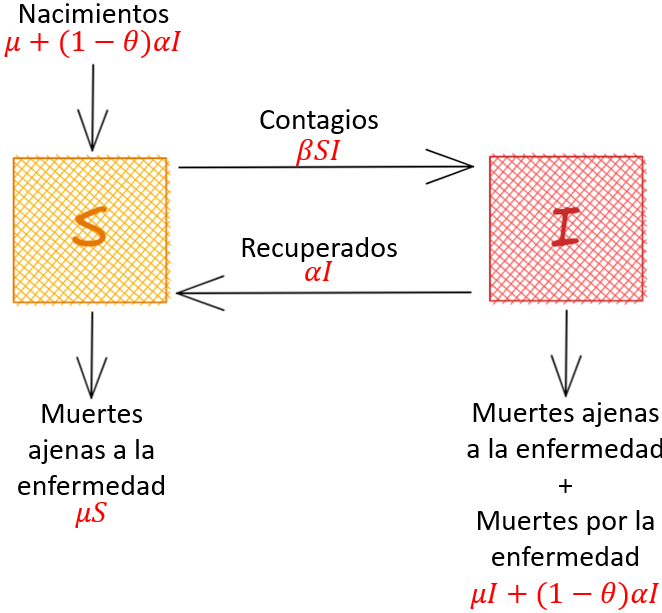
\includegraphics[width=0.6\textwidth]{Imagenes/SIS_compartimientos.PNG}
            \label{fig:diagrama SIS}
        \end{figure}
        \begin{equation*}\label{eq:Modelo SIS}
            \left\{\begin{array}{l}
                S' = \mu(1 - S) + (1 - \theta)\alpha I - \beta S I \\
                I' = \beta S I - (1 - \theta)\alpha I - \mu I
            \end{array}\right.
        \end{equation*}
        \begin{equation*}
            \mathcal{R}_0 = \frac{\beta}{\alpha(1-\theta)+\mu}
        \end{equation*}
    \end{block}
\end{minipage}
\hfill
\begin{minipage}{0.47\textwidth}
\begin{block}{Modelo SIR}
    \begin{figure}[h]
        \centering
        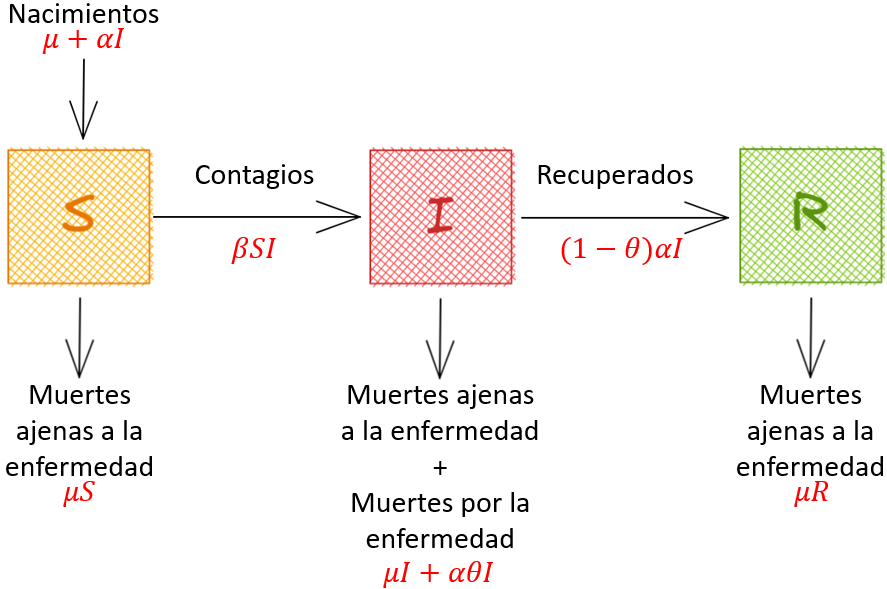
\includegraphics[width=0.9\textwidth]{Imagenes/SIR_compartimientos.PNG}
        \label{fig:diagrama SIR}
    \end{figure}
    \begin{equation*}\label{eq:Modelo SIR}
    \left\{\begin{array}{l}
        S' = \mu(1 - S) + \alpha\theta I - \beta S I \\
        I' = \beta S I - \mu I - \theta\alpha I - (1 - \theta)\alpha I \\
        R' = \alpha I - \alpha\theta I - \mu R
    \end{array}\right.
    \end{equation*}
    \begin{equation*}
        \mathcal{R}_0 = \frac{\beta}{\alpha+\mu}
    \end{equation*}
\end{block}
\end{minipage}
\end{frame}

\subsection{Nociones de topología}
\begin{frame}{Nociones de topología}
\textbf{Definición:} Una \textit{topología} sobre un conjunto $X$ es una colección $\tau$ de subconjuntos de $X$ que satisface las siguientes condiciones:
\begin{enumerate}
    \item $\emptyset$ y $X$ están en $\tau$,
    \item si $A,B\in\tau$, entonces $A\cap B\in\tau$, y 
    \item la unión de cualquier subcolección de $\tau$ esta en $\tau$.
\end{enumerate}

\textbf{Definición:} Una \textit{base} para una topología sobre un conjunto $X$ es una colección $\mathcal{B}$ de subconjuntos de $X$ tales que:
\begin{enumerate}
    \item Para todo $x\in X$, existe $B\in\mathcal{B}$ tal que $x\in B$, y
    \item dados $B_1,B_2\in\mathcal{B}$, existe $B_3\in\mathcal{B}$ tal que $B_3\subseteq B_1\cap B_2$.
\end{enumerate}

\textbf{Definición:} Sean $X$ un espacio topológico y $x\in X$. Diremos que un subconjunto $V$ de $X$ es una \textit{vecindad} de $x$ si existe un abierto $A$ tal que $x\in A\subseteq V$. Denotaremos por $\mathcal{V}(x)$ a la familia de todas las vecindades de $x$.

\textbf{Teorema:} Un subconjunto $A$ de un espacio topológico $X$ es un conjunto abierto si, y solo si es vecindad de cada uno de los puntos que contiene.
\end{frame}

\begin{frame}{Nociones de topología}
\textbf{Proposición:} Sea $X$ un espacio topológico, entonces para cada $x\in X$:
\begin{enumerate}
    \item Si $U\in\mathcal{V}(x)$, entonces $x\in U$,
    \item si $U,V\in\mathcal{V}(x)$, entonces $U\cap V\in\mathcal{V}(x)$,
    \item para cada $U\in\mathcal{V}(x)$, existe $V\in\mathcal{V}(y)$ tal que $U\in\mathcal{V}(y)$ para cada $y\in V$, y 
    \item si $U\in\mathcal{V}(x)$ y $U\subseteq V\subseteq X$ entonces $V\in\mathcal{V}(x)$.
\end{enumerate}

\textbf{Definición:} Para un punto $x$ en un espacio topológico $X$ un subconjunto $\mathcal{B}(x)$ de $\mathcal{V}(x)$ es un \textit{sistema fundamental de vecindades de $x$} sí para cada $V\in\mathcal{V}(x)$, existe $B\in\mathcal{B}(x)$ tal que $B\subseteq V$. Los elementos de $\mathcal{B}(x)$ son llamados \textit{vecindades (o entornos) básicos} de $x$.

\textbf{Definición:} Una \textit{vecindad minimal de} $x$ es la intersección de todas las vecindades de $x$. Lo denotaremos como $U_x$.

\textbf{Proposición:} La unión de todas las vecindades minimales $U_x$ para $x\in X$ forma una base para la topología de $X$. Esta base es llamada \textit{base minimal}.
\end{frame}

\begin{frame}{Nociones de topología}
\textbf{Definición:} Un \textit{conjunto preordenado finito} es un conjunto finito con una relación transitiva y reflexiva. Definiremos el la relación de orden parcial $x\preceq y$ si $x\in U_y$.

\textbf{Definición:} Un elemento $x$ en un conjunto parcialmente ordenado es llamado un maximal si $y\succeq x$ implica $y=x$, y es un máximo si $y\preceq x$ para todo $y\in X$.

\textbf{Definición:} Un espacio topológico $X$ es $T_0$ si para cada par de puntos $x,y\in X$ con $x\neq y$, existe $V\in\mathcal{V}(x)$ tal que $y\notin V$.

\textbf{Definición:} Un espacio topológico $X$ que tiene un sistema fundamental de vecindades numerable en cada uno de sus puntos se dice que satisface el primer axioma de numerabilidad o simplemente que es uno-numerable.
\end{frame}

\subsection{Autómatas celulares}
\begin{frame}{Autómatas Celulares}
Podemos pensar en un autómata celular como un conjunto de células que tienen diferentes comportamientos en el tiempo y que interactúan entre sí, de la misma manera que en sistema biológico de donde se obtiene su nombre.

La implementación computacional de un autómata celular por lo general se hace sobre matrices, por lo que el sistema que se quiere modelar se describe sobre una malla de tamaño regular.

\begin{figure}[h]
  \centering
    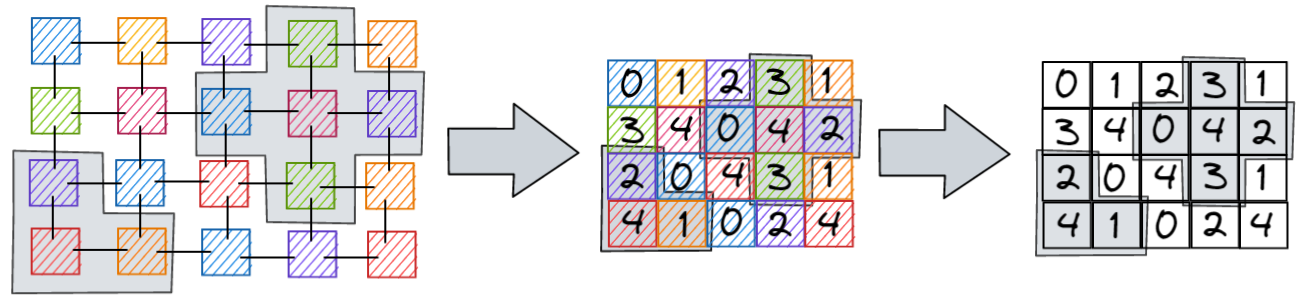
\includegraphics[width=1\textwidth]{Imagenes/ACaMatriz.PNG}
  \caption{Implementación computacional clásica de un autómata celular}
  \label{fig:AC a matriz}
\end{figure}
\end{frame}

\section{Modelos epidemiológicos en autómatas celulares}
\subsection{Interacciones e impactos sociales}
\begin{frame}{Interacciones e impactos sociales}
A diferencia del trabajo realizado en \cite{populationDensity} en el que cada celda representaba una región, consideraremos a cada división como un único individuo que será dotado de un conjunto de cualidades como estado de salud, edad, vecinos, etc.

Pensemos por un momento en las características que hay detrás de relación cercana entre individuos o células. Denotaremos la relación entre células con el símbolo $\thicksim$ y de ese modo tenemos que:

\begin{itemize}
    \item Todas las células están en contacto con ellas mismas, por lo que para cada célula $x$ se cumple $x \thicksim x$.
    \item Si una célula estuviera en contacto con alguna otra entonces esa célula estaría en contacto con la primera, es decir, $x\thicksim y$ implica $y\thicksim x$.
    \item Si una célula interactúa con otras dos no implica necesariamente que estas interactúen entre sí, por lo que $x\thicksim y$ y $x\thicksim z$ no implican que $y\thicksim z$.
\end{itemize}
\end{frame}

\begin{frame}{Interacciones e impactos sociales}
\textbf{Ejemplo:} Consideremos al conjunto $A=\{a,b,c,d\}$ y una sub-colección definida por $\mathcal{B} = \{\{a\},\{b\},\{c\},\{d\},\{a,c,d\}, \{b,c\}, \{b,d\}\}$ de $A$. Claramente se obtienen las siguientes relaciones

$$\begin{array}{cccc}
    a\thicksim a, & b\thicksim b, & c\thicksim c, & d\thicksim d, \\ 
    a\thicksim c, & a\thicksim d, & b\thicksim c, & b\thicksim d,
\end{array}$$

junto con sus relaciones simétricas equivalentes. 

\textbf{Definición:} Definimos el \textit{grado de impacto} entre dos puntos $a$ y $b$ como la menor cantidad de interacciones necesaria para llegar de $a$ a $b$. Para reconocer el grado de impacto entre dos puntos usaremos la notación $a\thicksim_n b$ donde $n\in\mathbb{N}$ denota la menor cantidad de interacciones entre $a$ y $b$.

Si retomamos el ejemplo anterior, podremos identificar los siguientes grados de impacto:

$$\begin{array}{cccc}
    a\thicksim_0 a, & b\thicksim_0 b, & c\thicksim_0 c, & d\thicksim_0 d, \\ 
    a\thicksim_1 c, & a\thicksim_1 d, & b\thicksim_1 c, & b\thicksim_1 d, \\
    a\thicksim_2 b, & c\thicksim_2 d.
\end{array}$$
\end{frame}

\begin{frame}{Interacciones e impactos sociales}
\textbf{Teorema:} Los grados de impacto de una célula $x$ definen un sistema fundamental de vecindades en la topología discreta.

\begin{proof}
Para una célula $x$ y una familia de vecindades $\mathcal{V}(x)$ defina el conjunto $A_0=\{x\}$, como el conjunto de puntos con grado de impacto con $x$ es igual a cero y de manera recursiva defina a los conjuntos $A_k$ como los conjuntos cuyos elementos tienen grado de impacto con $x$ igual o menor a $k$. Claramente $A_i\subseteq A_j$ para $0\leq i\leq j$ y de ese modo $A_i\in\mathcal{V}(x)$ para $i=0,1,\cdots,n$.

Defina la colección $\mathcal{A}=\{A_0,A_1,\cdots,A_k,\cdots,A_N\}$ como la familia de conjuntos encajados definidos por el grado de impacto con $x$. Dado que por hipótesis estamos sobre la topología discreta podemos afirmar que para todo $V\in\mathcal{V}(x)$ el conjunto $A_0\subseteq V$ y de ese modo por la definición de sistema fundamental de vecindades concluimos que la colección $\mathcal{A}$ es un sistema fundamental de vecindades de $x$.
\end{proof}

\textbf{Proposición:} Sea $x\in\mathcal{L}$ una célula y sea $\mathcal{A}$ la familia de conjuntos encajados definidos por el grado de impacto con $x$. Se cumplen las siguientes propiedades:

\begin{enumerate}
    \item El conjunto $\mathcal{A}$ posee elemento mínima igual a $A_0=\{x\}$,
    \item $\mathcal{A}$ es un conjunto ordenado finito con el orden de la contenencia,
    \item $\mathcal{L}$ es un espacio $T_0$, y
    \item $\mathcal{L}$ es un espacio uno-numerable.
\end{enumerate}
\end{frame}

\subsection{Reglas de evolución}
\begin{frame}{Reglas de evolución}
\begin{alertblock}{Notación}
\begin{itemize}
    \item Denotaremos por $\pi^t(x)$ al estado de la célula $x$ en el momento $t$.
    \item Para describir la cantidad de vecinos de una célula $x$ que tengan un estado $K$ en un momento $t$ usaremos el símbolo $\sigma_K^t(x)$.
    \item Usaremos los símbolos $\mathcal{S}^t,\mathcal{I}^t,\mathcal{R}^t$ y $\mathcal{D}^t$ para denotar a los conjuntos de células susceptibles, infectadas, recuperadas y muertas respectivamente en el espacio $\mathcal{L}$ en el tiempo $t$. De manera formal
    $$\mathcal{S}^t=\{x\in\mathcal{L}:\pi^t(x)=S\},$$
    y de manera análoga se definen los conjuntos $\mathcal{I}^t,\mathcal{R}^t$ y $\mathcal{D}^t$. Note que $$\mathcal{S}^t\cup\mathcal{I}^t\cup\mathcal{R}^t\cup\mathcal{D}^t=\mathcal{L}\text{ para todo tiempo }t.$$
\end{itemize}
\end{alertblock}
\end{frame}

\subsection{Modelos SIS y SIR simples}
\begin{frame}{Modelos SIS y SIR simples}
Recordemos que para las tasas de infección $\beta$ y de recuperación $\alpha$ los modelos SIS y SIR simples nos afirman que para $\mathcal{R}_0=\frac{\beta}{\alpha}>1$, la enfermedad será endémica. Analicemos los siguientes escenarios para cada estado:

\begin{itemize}
    \item Si $\mathcal{R}_0>1$, la probabilidad de que un individuo susceptible se enferme luego de tener contacto con un infectado es más alta que la probabilidad de continuar susceptible a la enfermedad; caso contrario ocurre sí $\mathcal{R}_0<1$. Esta probabilidad de adquirir la enfermedad depende en gran medida de la cantidad de individuos infectados que la célula tenga en su vecindad. 
    
    \item La recuperación de los individuos infectados no se ve afectada por la cantidad de contactos con otras células y en lugar de eso depende completamente de la tasa de recuperación $\alpha$.
    
    \item Para el estado de inmunidad en el modelo SIR, supondremos que los individuos que posean este estado se mantendrán inmunes. Esto quiere decir que la transformación para individuos recuperados será constante.
\end{itemize}
\end{frame}

\begin{frame}{Modelos SIS y SIR simples}
\textbf{Definición:} Dada una célula $x$ en un conjunto $\mathcal{L}$ definimos la regla de evolución para el modelo SIS como:
\begin{equation}
    \phi_{SIS}^t(x)=\left\{\begin{array}{ll}
        S & \text{si }\pi^t(x)=S\text{ y }\rho\leq\frac{\beta}{\alpha}\frac{\pi_I^t(x)}{\#\mathcal{V}(x)}, \\
        I & \text{si }\pi^t(x)=S\text{ y }\rho>\frac{\beta}{\alpha}\frac{\pi_I^t(x)}{\#\mathcal{V}(x)}, \\
        I & \text{si }\pi^t(x)=I\text{ y }\rho>\alpha,\\
        S & \text{si }\pi^t(x)=I\text{ y }\rho\leq\alpha.
    \end{array}\right.
\end{equation}
Donde $\rho\in\mathcal{U}_{[0,1]}$.
    
\textbf{Definición:} Dada una célula $x$ en un conjunto $\mathcal{L}$ definimos la regla de evolución para el modelo SIR como:
\begin{equation}
    \phi_{SIR}^t(x)=\left\{\begin{array}{ll}
        S & \text{si }\pi^t(x)=S\text{ y }\rho\leq\frac{\beta}{\alpha}\frac{\pi_I^t(x)}{\#\mathcal{V}(x)}, \\
        I & \text{si }\pi^t(x)=S\text{ y }\rho>\frac{\beta}{\alpha}\frac{\pi_I^t(x)}{\#\mathcal{V}(x)}, \\
        I & \text{si }\pi^t(x)=I\text{ y }\rho>\alpha,\\
        R & \text{si }\pi^t(x)=I\text{ y }\rho\leq\alpha, \\
        R & \text{si }\pi^t(x)=R.
    \end{array}\right.
\end{equation}
Con $\rho\in\mathcal{U}_{[0,1]}$.
\end{frame}

\subsection{Modelos con natalidad y mortalidad}
\begin{frame}{Modelos con natalidad y mortalidad}
Para estos modelos debemos tener en cuenta el estado de la célula central junto con su edad y el estado de sus vecinos, de modo que 
$$Dom(\phi_\mu)=\Sigma_x\times K\times\overbrace{\Sigma\times\cdots\times\Sigma}^N\text{, con }K=\{1,2,\cdots,100\},$$
si suponemos que la edad de la célula $x$ puede ir de 1 a 100 unidades temporales (semanas, meses, años, etc.).

Podemos pensar envejecimiento de las células, esto con el objetivo de analizar el impacto de una enfermedad sobre los individuos de un sistema en diferentes etapas de su "vida". 
$$Ran(\phi_\mu)=\Sigma_x\times K.$$

Dado que estamos trabajando sobre poblaciones de tamaño constante la manera en la que interpretaremos el nacimiento de una célula será con la ocupación del espacio que deja una que muere. Para esto identificaremos a los espacios que dejan las células que mueren con el estado $D$ y una edad cero.
\end{frame}

\begin{frame}{Modelos con natalidad y mortalidad}
\textbf{Definición:} Sea $x$ una célula en un conjunto $\mathcal{L}$, $M$ un modelo epidemiológico y $T$ una unidad temporal (días, meses, años, etc.). Definimos la regla de evolución con nacimientos y muertes para $M$ como:
\begin{equation}
    \mu_{M,T}^t(x)=\left\{\begin{array}{ll}
        D,0 & \text{si }t\not\equiv 0 \text{ (modulo }T\text{), }\pi^t(x)\in\{S,I,R\}\text{ y }\rho\leq\omega_k, \\
        D,0 & \text{si }\pi^t(x)=D\text{ y }\rho>b,\\
        S,1 & \text{si }\pi^t(x)=D\text{ y }\rho\leq b,\\
        \phi_M^t(x),E^t(x) & \text{si }t\not\equiv 0 \text{ (modulo }T),\\
        \phi_M^t(x),E^t(x)+1 & \text{si }t\equiv 0 \text{ (modulo }T),
    \end{array}\right.
\end{equation}
donde $\omega_k$ es la probabilidad de morir por causas ajenas a la enfermedad para las edades en la partición k-ésima del intervalo $[0,100]$, $b$ es la tasa de natalidad, $\phi_M^t$ es la regla de evolución del modelo epidemiológico, $E^t(x)$ denota la edad de la célula $x$ en el momento $t$ y $\rho\in\mathcal{U}_{[0,1]}$.
\end{frame}

\subsection{Modelos con muerte por enfermedad}
\begin{frame}{Modelos con muerte por enfermedad}
Al igual que en la sección anterior, realizaremos una partición sobre el intervalo $[0,100]$ y definiremos una probabilidad $\theta_k$ que indique la probabilidad de morir a causa de la enfermedad en la k-ésima partición. De manera formal:

\textbf{Definición:} Sea $x$ una célula en un conjunto $\mathcal{L}$, $M$ un modelo epidemiológico y $T$ una unidad temporal (días, meses, años, etc.). Definimos la regla de evolución con muerte por enfermedad para $M$ como:
\begin{equation}
    \theta_{M,T}^t(x)=\left\{\begin{array}{ll}
        D,0 & \text{si }\pi^t(x)=I\text{ y }\rho\leq\theta_k, \\
        \mu_{M,T}^t(x) & \text{en otro caso.}
    \end{array}\right.
\end{equation}
Donde $\theta_k$ es la probabilidad de morir por la enfermedad para los individuos con una edad en el intervalo k-ésimo de la partición del intervalo $[0,100]$, $\mu_{M,T}^t$ es la regla de evolución para modelos con nacimientos y muertes y $\rho\in\mathcal{U}_{[0,1]}$.
\end{frame}

\section{Referencias}
\begin{frame}[allowframebreaks]{Referencias}
\bibliographystyle{plain} % apalike
\bibliography{BibliMSc}
\end{frame}

\end{document}